\documentclass[11pt,a4paper]{article}

\usepackage[margin=1in]{geometry}
\usepackage{amsmath,amssymb}
\usepackage{booktabs}
\usepackage{graphicx}
\usepackage{hyperref}
\usepackage{microtype}

\hypersetup{
  colorlinks=true,
  linkcolor=blue,
  citecolor=blue,
  urlcolor=blue
}

\title{A Mass-Stabilized, Non-Hierarchical \texttt{AAAbbb} Periodic Three-Body Family with Nonzero Angular Momentum}
\author{gawydion\thanks{Email: \texttt{gawydion@gmail.com}; Code and dataset: \url{https://github.com/gawydion/3-body-orbits}}}
\date{November 2026}

\begin{document}
\maketitle

\begin{abstract}
We report a periodic orbit family of the planar Newtonian three-body problem with nonzero angular momentum ($L \neq 0$).
The family has the canonical $S_3$ Montgomery shape-sphere free-group word \texttt{AAAbbb} (length 6).
In the inertial frame, the pairwise winding numbers are $(w_{12}, w_{13}, w_{23}) = (-5, -5, -2)$.
In the co-rotating frame of bodies 2 and 3, body 1 makes three prograde loops around body 2 and three prograde loops around body 3.

At equal masses ($m_1 = m_2 = m_3 = 1$) and zero precession ($\alpha = 0$), the orbit is linearly unstable ($k_1 = +3.5689$, largest Floquet multiplier $|\lambda| = 3.268$).
We find two mechanisms that produce full three-dimensional (3D) linear stability ($|k_1|, |k_2|, |k_z| < 2$).
First, reducing the mean companion mass $(m_2 + m_3)/2$ below $m_1$ opens a broad two-dimensional (2D) mass-space stability island.
Every planar-stable orbit in this island is also vertically stable ($|k_z| < 0.6$).
The linear 3D stability margin reaches $1.5963$ at $m = [1, 0.94, 0.71]$.
The island contains all-distinct-mass orbits such as \texttt{2D-DEM-002} at $m = [1, 0.9, 0.8]$ (margin $1.2061$).
It also contains isosceles orbits on $m_2 = m_3 \in [0.683, 0.939]$ and narrow peninsulas that pass through $m = [1, 1, 0.88]$ (margin $0.4267$).
Second, at equal masses $m = [1, 1, 1]$, adding frame precession $\alpha/\pi \in [0.061, 0.096]$ produces full-3D linearly stable $q$-fold inertial rosettes \texttt{(AAAbbb)\^{}q} for $q \in \{11, 12, 13, 14, 15, 16\}$.

We trace the isosceles branch $m = [\varepsilon, 1, 1]$ to the restricted limit $\varepsilon \to 0$.
It connects smoothly to a 2:1 resonant orbit of the equal-mass elliptic restricted three-body problem ($e = 0.092555$) and then to a violently unstable doubly-symmetric 3+3 exchange orbit of the circular Copenhagen problem ($C_J = 3.696245$, $|\lambda| \approx 337.8$).
We verify nine benchmark orbits in 128-bit quad precision using a 16th-order symplectic Gauss--Legendre integrator (return error $\le 4.1 \times 10^{-31}$, canonical symplecticity error $\le 3.4 \times 10^{-28}$).
Full-3D symplectic integrations over $10{,}000$ periods confirm bounded motion under 3D velocity perturbations of $10^{-5}$ and $10^{-4}$, while the equal-mass inertial control orbit breaks apart in 10 periods.
We check the \texttt{threebodyorbits.com} Atlas ($3{,}942$ orbits), \texttt{/hunt/garden} ($82{,}032$ loops), and major published $L = 0$ and $L \neq 0$ catalogs, and find zero matches to \texttt{AAAbbb}.
\end{abstract}

\section{Introduction}
Most known periodic orbits of the general planar three-body problem fall into two groups.
The first group contains hierarchical orbits with nonzero angular momentum ($L \neq 0$), such as the Broucke--Hadjidemetriou--H\'enon (BHH) family and its satellites \cite{Broucke1975,BrouckeBoggs1975,Hadjidemetriou1975,Henon1976,Jankovic2016,LiLiao2020}.
In those orbits, one close binary pair stays intact while a third body orbits outside it, and the Montgomery free-group word has the form $A^k$.
The second group contains non-hierarchical exchange orbits with zero angular momentum ($L = 0$), such as the figure-eight orbit and its unequal-mass extensions \cite{Moore1993,ChencinerMontgomery2000,Suvakov2013,LiLiao2017,LiJingLiao2018}.

Linearly stable, non-hierarchical, unequal-mass periodic orbits with $L \neq 0$ are rare.
Li, Li \& Liao \cite{LiLiLiao2021} reported one such family of $13{,}315$ stable orbits.
That family belongs to the length-10 Moth~I class \texttt{ABAbaBABab}, has small scale-invariant angular momentum $\Lambda = |L|\sqrt{|E|} \in [0.006, 0.058]$, and has close passages near $r_{\min} \approx 0.016$.

In this note, we present a second, distinct non-hierarchical $L \neq 0$ family with canonical free-group word \texttt{AAAbbb}.
This family has large angular momentum ($\Lambda \in [1.28, 2.24]$), wide minimum separations ($r_{\min} \in [0.163, 0.246]$), and deep full-3D linear stability across a broad region of mass space.

\section{Equations of Motion and Numerical Methods}
We study three point masses $m_1, m_2, m_3$ under Newtonian gravity with $G = 1$ in the center-of-mass frame ($\sum m_i \mathbf{r}_i = \mathbf{0}$, $\sum m_i \mathbf{v}_i = \mathbf{0}$).
The equations of motion are
\begin{equation}
\ddot{\mathbf{r}}_i = \sum_{j \neq i} m_j \frac{\mathbf{r}_j - \mathbf{r}_i}{\|\mathbf{r}_j - \mathbf{r}_i\|^3}, \qquad i \in \{1, 2, 3\}.
\end{equation}
We set $m_1 = 1$ and normalize the spatial scale by $x_1(0) = -1$.
Every orbit in this family starts on the collinear perpendicular crossing subspace at $t = 0$:
\begin{equation}
y_i(0) = 0, \qquad \dot{x}_i(0) = 0, \qquad i \in \{1, 2, 3\}.
\end{equation}
We shoot to the half-period $t = T/2$ in a rotated frame $R(-\alpha)$ and solve four boundary equations:
\begin{equation}
y_1^{\text{rot}}(T/2) = 0, \quad y_2^{\text{rot}}(T/2) = 0, \quad \dot{x}_1^{\text{rot}}(T/2) = 0, \quad \dot{x}_2^{\text{rot}}(T/2) = 0.
\end{equation}
Time-reversal symmetry guarantees closure after one full period $T$ with total rotation $2\alpha$.
Setting $\alpha = 0$ gives an exact inertial periodic orbit.
Setting $\alpha = \pi/q$ gives a relative periodic orbit (RPO) that closes in the inertial frame after $q$ periods ($T_{\text{inert}} = qT$).

To verify each benchmark orbit without double-precision limits, we use an independent C++20 solver (\texttt{src/confirm\_aaabbb.cpp}) in 128-bit quad precision (\texttt{\_\_float128}, about 34 decimal digits).
The solver uses an 8-stage, 16th-order symplectic Gauss--Legendre integrator (\texttt{GL16}) \cite{Hairer2006}.
We compute the Butcher tableau directly from the roots of the Legendre polynomial $P_8$ using factored Lagrange quadrature.
Self-tests give order-16 quadrature error $3.85 \times 10^{-34}$, symplecticity error $|b_i A_{ij} + b_j A_{ji} - b_i b_j|_{\max} = 6.62 \times 10^{-35}$, and a two-body Kepler ($e = 0.6$) one-period return error of $9.82 \times 10^{-32}$.

We compute linear stability from exact analytical variational equations integrated over one full period $T$: the $12 \times 12$ planar monodromy matrix $M_p$ and the $6 \times 6$ out-of-plane vertical matrix $M_z$.
We verify canonical symplecticity $\|S^\top J S - J\|_\infty$ directly, where $S = D M_{\text{rot}} D^{-1}$ converts velocities to canonical momenta $p_i = m_i v_i$.
We extract the three nontrivial Broucke--Floquet stability indices $(k_1, k_2, k_z)$ from trace invariants of $M_{\text{rot}}$ and $M_z$.
An orbit is full-3D linearly stable when $k_1, k_2, k_z$ are real and lie strictly inside $(-2, 2)$.
We define the 3D linear stability margin as
\begin{equation}
M_{3\text{D}} = 2 - \max(|k_1|,\, |k_2|,\, |k_z|).
\end{equation}

To test nonlinear stability, we apply a zero-momentum 3D velocity kick $\Delta \mathbf{v}_1 = \frac{\delta}{\sqrt{3}}(1, 1, 1)$ (compensated equally on bodies 2 and 3).
We then integrate the full 18D system for $10{,}000$ periods using a fixed-step 4-stage, 8th-order symplectic Gauss--Legendre integrator (\texttt{GL8}, $1{,}200$ steps per period).

\section{Geometry, Symmetries, and Restricted-Problem Origin}

\subsection{Co-Rotating 3 + 3 Shuttle-Exchange Motion}
Figure~\ref{fig:corot} shows the flagship orbit \texttt{AAAbbb-DEM002} (\texttt{2D-DEM-002}, $m = [1, 0.9, 0.8]$) in both the inertial frame and the co-rotating frame of bodies 2 and 3.

\begin{figure}[t]
  \centering
  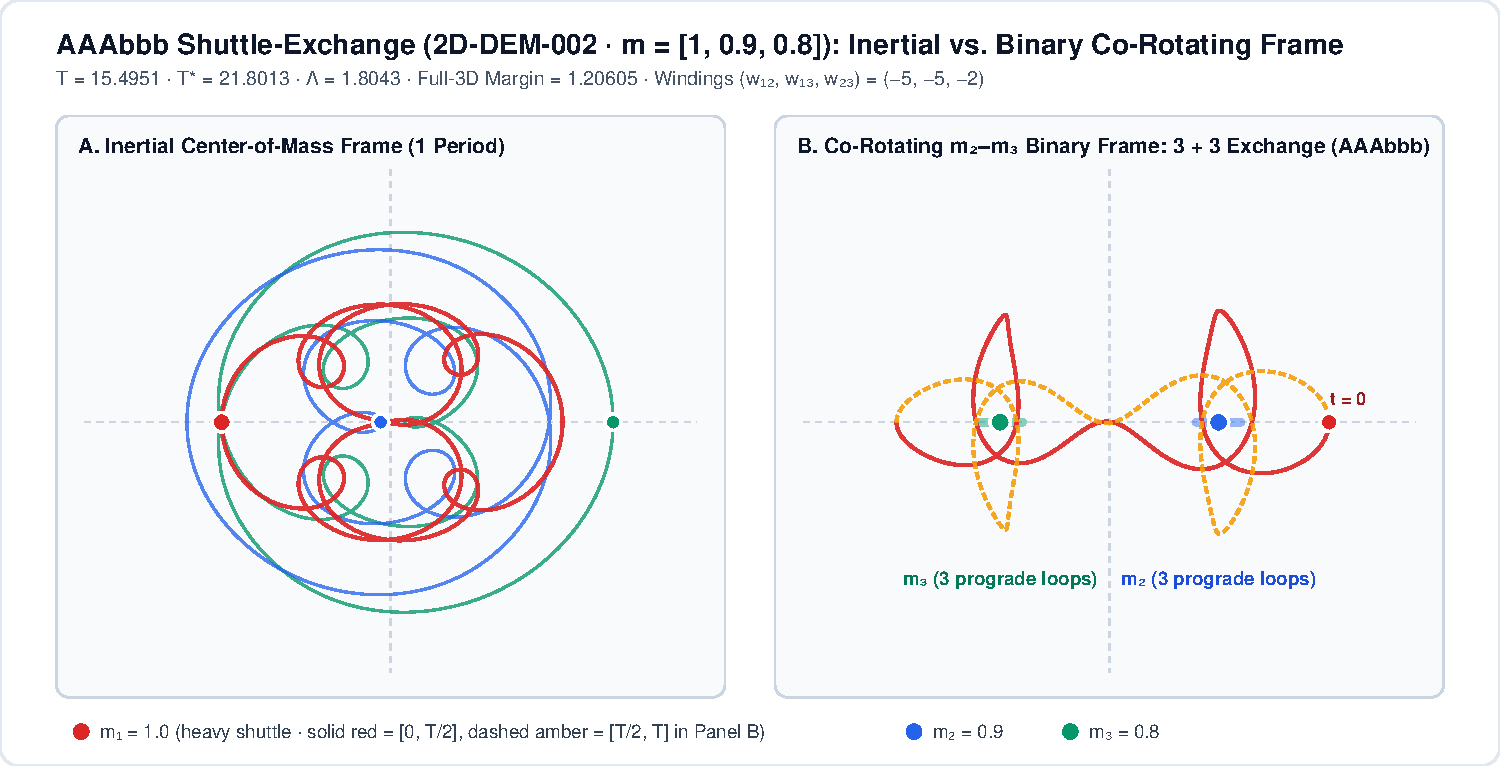
\includegraphics[width=\textwidth]{fig1_corotating.pdf}
  \caption{Flagship orbit \texttt{AAAbbb-DEM002} ($m = [1, 0.9, 0.8]$, $T = 15.4951$, $M_{3\text{D}} = 1.2061$). Left: inertial center-of-mass frame over one period. Right: co-rotating frame aligned with the body~2--body~3 axis. Body~1 makes three prograde loops around body~2 (\texttt{AAA}) and three prograde loops around body~3 (\texttt{bbb}).}
  \label{fig:corot}
\end{figure}

Over one inertial period, the pairwise winding numbers are $(w_{12}, w_{13}, w_{23}) = (-5, -5, -2)$.
Bodies 2 and 3 orbit each other two times clockwise while staying well separated ($r_{23} \in [1.290, 1.948]$).
In the co-rotating frame of the body~2--body~3 pair, the relative windings are
\begin{equation}
(w_{12} - w_{23},\, w_{13} - w_{23}) = (-3,\, -3).
\end{equation}
Body~1 acts as a shuttle.
It completes three prograde loops around body~2, crosses the central saddle between bodies 2 and 3, and completes three prograde loops around body~3.
This double-trifoil geometry yields the canonical $S_3$ Montgomery free-group word \texttt{AAAbbb} (length 6).
Both exchange pairs span wide distance ratios: $r_{12} \in [0.2321, 2.2235]$ and $r_{13} \in [0.1893, 2.3170]$.

When $m_2 = m_3$, the orbit gains two additional symmetries:
\begin{enumerate}
  \item Half-period companion exchange with $180^\circ$ rotation: $\mathbf{r}_1(T/2) = -\mathbf{r}_1(0)$, $\mathbf{r}_2(T/2) = -\mathbf{r}_3(0)$, and $\mathbf{r}_3(T/2) = -\mathbf{r}_2(0)$.
  \item Exact isosceles triangle configurations ($r_{12} = r_{13}$) at $t = T/4$ and $t = 3T/4$, where body~1 crosses the perpendicular bisector of the body~2--body~3 axis at maximum companion separation.
\end{enumerate}

\subsection{Connection to the Copenhagen Restricted Three-Body Problem}
We continue the isosceles exchange branch in Jacobi coordinates ($x_2(0) - x_3(0) = 1$) in both directions from equal masses $m = [1, 1, 1]$:
\begin{enumerate}
  \item \textbf{Restricted limit $m = [\varepsilon, 1, 1]$ ($\varepsilon \to 0$):} The branch continues smoothly to $\varepsilon = 0$ with no collision or bifurcation. At $\varepsilon = 0$, bodies 2 and 3 move on a Kepler ellipse with eccentricity $e = 0.09255493$. Body~1 moves on a 2:1 resonant periodic orbit ($T / T_{\text{Kep}} = 2$) of the equal-mass elliptic restricted three-body problem (ER3BP). This ER3BP orbit is Krein-unstable ($k = (-0.5144, \pm 35.234i)$, $|\lambda| \approx 35.2$).
  \item \textbf{Circular Copenhagen limit ($e \to 0$ at $m_1 = 0$):} Continuing the ER3BP orbit from $e = 0.092555$ to $e = 0$ reaches a doubly-symmetric 3+3 prograde exchange orbit of the circular Copenhagen problem \cite{Henon1965} ($m_2 = m_3 = 1/2$, $a = 1$, $T_{\text{rot}} = 4\pi$). Its initial state is $x_0 = 0.95455981$ and $\dot{y}_{\text{rot}} = +0.31994239$, with Jacobi constant $C_J = 3.69624503$. This circular limit is strongly hyperbolic, with H\'enon stability index $a_{\text{H\'enon}} = +168.9022$ ($|\lambda| \approx 337.8$).
  \item \textbf{Lower mass fold $m = [1, \mu, \mu]$ ($\mu$ decreasing):} Decreasing $\mu$ below $1$ enters stability at $\mu \approx 0.9396$, leaves stability at $\mu \approx 0.6825$ ($k_1 \to +2$), and ends at a smooth saddle-node fold at $\mu_{\min} \approx 0.45746$ ($r_{\min} \approx 0.2144$). The family does not reach the planetary limit $\mu \to 0$.
\end{enumerate}

\section{Dual Full-3D Stabilization Mechanisms}

\subsection{Two-Dimensional Mass-Space Stability Island ($\alpha = 0$)}
We map the inertial family ($\alpha = 0$) on a uniform $0.02$-step grid over $(m_2, m_3) \in [0.54, 1.06]^2$ with $m_1 = 1$ (729 grid points; Figure~\ref{fig:island}).
The phase diagram is symmetric under $m_2 \leftrightarrow m_3$ and contains 310 full-3D linearly stable grid points (\texttt{S3}), 224 Krein-unstable points (\texttt{K}), and 195 hyperbolically unstable points (\texttt{H}).

\begin{figure}[t]
  \centering
  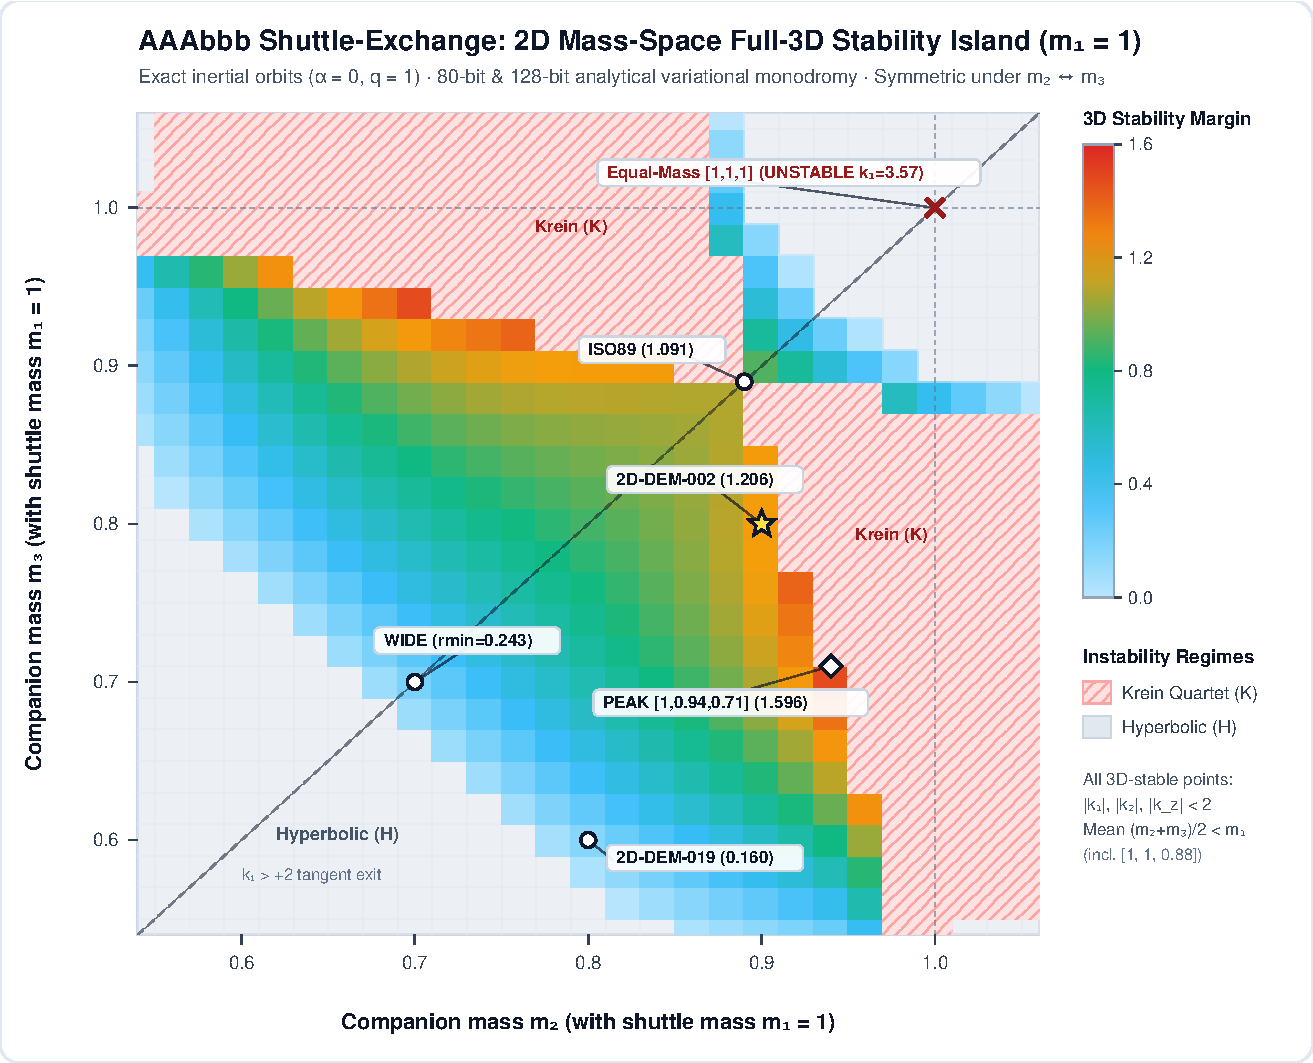
\includegraphics[width=0.92\textwidth]{fig2_stability_island.pdf}
  \caption{Two-dimensional mass-space stability diagram for the inertial \texttt{AAAbbb} family ($m_1 = 1$, $\alpha = 0$, 729 points on a $0.02$-step grid). Color shows the full-3D linear stability margin $M_{3\text{D}}$. Hatched pink marks Krein-quartet instability (\texttt{K}). Light gray marks hyperbolic instability (\texttt{H}). Every planar-stable point is also vertically stable ($|k_z| < 0.6$).}
  \label{fig:island}
\end{figure}

Key properties of the stability island are:
\begin{itemize}
  \item \textbf{Automatic 3D vertical stability:} Every planar-stable point in the island satisfies $|k_z| < 0.6$. No vertical instability occurs anywhere inside the planar stability region.
  \item \textbf{Mean-mass condition and narrow peninsulas:} Along the symmetry diagonal $m_2 = m_3$, full-3D stability spans $\mu \in [0.683, 0.939]$ and peaks at \texttt{AAAbbb-ISO89} ($m = [1, 0.89, 0.89]$, $M_{3\text{D}} = 1.0909$). Off the diagonal, stability holds across a broad region where $(m_2 + m_3)/2 < m_1$. Two narrow stable peninsulas around $m_3 \approx 0.88$ (and $m_2 \approx 0.88$) thread between the upper hyperbolic region and the lower Krein tongue past $m_2 = 1$. Independent 80-bit checks confirm full-3D stability at the two-equal-mass point $m = [1, 1, 0.88]$ ($M_{3\text{D}} = 0.42669$, symplecticity error $8.7 \times 10^{-11}$) and out to $m = [1, 1.06, 0.88]$ ($M_{3\text{D}} = 0.00636$).
  \item \textbf{Symmetry-protected crossing vs.\ Krein cliff:} Along $m_2 = m_3$, the two planar stability indices $k_1$ and $k_2$ cross near $\mu \approx 0.893$ without becoming complex because the two modes have opposite exchange parity. Breaking $m_2 = m_3$ opens this crossing into two Krein-quartet tongues (\texttt{K}). The global linear margin peaks right beside the Krein boundary at \texttt{AAAbbb-PEAK} ($m = [1, 0.94, 0.71]$, $M_{3\text{D}} = 1.59631$, $|k_1 - k_2| = 0.1147$).
\end{itemize}

\subsection{Equal-Mass Rotating-Frame Stabilization ($m = [1, 1, 1]$)}
Continuing the unstable equal-mass orbit ($m = [1, 1, 1]$, $\alpha = 0$) in frame precession angle $\alpha$ opens a full-3D linearly stable RPO window across $\alpha/\pi \in [0.061, 0.096]$.
Every rational value $\alpha/\pi = 1/q$ for $q \in \{11, 12, 13, 14, 15, 16\}$ yields a full-3D linearly stable equal-mass inertial rosette \texttt{(AAAbbb)\^{}q}.
The strongest closure is $q = 13$ (\texttt{AAAbbb-EQ-RPO13}), which has RPO margin $1.16261$ and exact full inertial ($13T$) margin $0.57216$.

\section{High-Precision Benchmarks and 10,000-Period 3D Survival}
Table~\ref{tab:quad} lists the 128-bit \texttt{GL16} verification metrics for nine benchmark orbits.
Every orbit passes canonical symplecticity to $\le 3.41 \times 10^{-28}$, energy conservation to $|dE| \le 1.19 \times 10^{-32}$, angular momentum conservation to $|dL| \le 2.70 \times 10^{-33}$, and independent \texttt{GL16} step-halving ($h$ vs.\ $h/2$) to $\le 5.07 \times 10^{-31}$.
On \texttt{AAAbbb-DEM002}, step-halving also verifies the Floquet indices $(k_1, k_2, k_z)$ to $9.02 \times 10^{-28}$.

\begin{table}[t]
  \centering
  \scriptsize
  \setlength{\tabcolsep}{3.5pt}
  \begin{tabular}{@{}llrrrrrrrrrr@{}}
    \toprule
    Orbit ID & Masses & $T$ & $T^*$ & $\Lambda$ & $k_1$ & $k_2$ & $k_z$ & $M_{3\text{D}}$ & $r_{\min}$ & Return err & Symp.\ err \\
    \midrule
    \texttt{AAAbbb-DEM002} & $[1,0.9,0.8]$ & 15.495142 & 21.801 & 1.804 & $+0.7940$ & $+0.2189$ & $-0.2568$ & \textbf{1.20605} & 0.1893 & $1.29\times10^{-31}$ & $7.36\times10^{-29}$ \\
    \texttt{AAAbbb-PEAK}   & $[1,0.94,0.71]$ & 16.334090 & 20.734 & 1.705 & $+0.4037$ & $+0.2890$ & $-0.2632$ & \textbf{1.59631} & 0.1714 & $2.49\times10^{-31}$ & $6.88\times10^{-29}$ \\
    \texttt{AAAbbb-DEEP}   & $[1,0.94,0.70]$ & 16.465102 & 20.532 & 1.687 & $+0.5238$ & $+0.1516$ & $-0.2585$ & \textbf{1.47617} & 0.1705 & $2.94\times10^{-31}$ & $7.76\times10^{-29}$ \\
    \texttt{AAAbbb-ISO89}  & $[1,0.89,0.89]$ & 14.638051 & 23.397 & 1.951 & $+0.9091$ & $+0.8753$ & $-0.3494$ & \textbf{1.09091} & 0.2009 & $4.12\times10^{-31}$ & $6.63\times10^{-29}$ \\
    \texttt{AAAbbb-ISO85}  & $[1,0.85,0.85]$ & 15.265692 & 21.826 & 1.807 & $+0.9656$ & $+0.0978$ & $-0.2401$ & \textbf{1.03439} & 0.2076 & $1.96\times10^{-31}$ & $8.71\times10^{-29}$ \\
    \texttt{AAAbbb-WIDE}   & $[1,0.70,0.70]$ & 18.360881 & 16.308 & 1.314 & $+1.8042$ & $-1.6447$ & $+0.2273$ & \textbf{0.19585} & 0.2429 & $6.72\times10^{-32}$ & $1.13\times10^{-28}$ \\
    \texttt{AAAbbb-DEM019} & $[1,0.80,0.60]$ & 19.054860 & 16.212 & 1.303 & $+1.8402$ & $-1.3431$ & $+0.1202$ & \textbf{0.15979} & 0.1970 & $4.13\times10^{-31}$ & $9.60\times10^{-29}$ \\
    \texttt{AAAbbb-EQ-UNST}& $[1,1,1]$ & 13.199687 & 27.925 & 2.372 & $+3.5689$ & $+0.9233$ & $-0.6184$ & unstable & 0.1860 & $1.67\times10^{-31}$ & $1.14\times10^{-28}$ \\
    \texttt{AAAbbb-EQ-RPO13}& $[1,1,1]$ ($q\!=\!13$) & 166.111724 & 27.352 & 2.371 & $+1.2374$ & $-1.4278$ & $-1.2965$ & \textbf{0.57216} & 0.1794 & $3.30\times10^{-29}$ & $1.72\times10^{-25}$ \\
    \bottomrule
  \end{tabular}
  \caption{128-bit \texttt{GL16} verification of nine \texttt{AAAbbb} benchmarks. For \texttt{AAAbbb-EQ-RPO13}, $T$, stability indices, $M_{3\text{D}}$, return error, and symplecticity error are given for the exact 13-fold inertial closure ($T_{\text{inert}} = 13 T_{\text{rpo}}$); $T^*$ and $\Lambda$ are given for one primitive RPO period ($T_{\text{rpo}} = 12.777825$).}
  \label{tab:quad}
\end{table}

Table~\ref{tab:lt} summarizes the $10{,}000$-period full-3D symplectic \texttt{GL8} perturbation tests.
These tests confirm an important physical distinction.
\texttt{AAAbbb-PEAK} and \texttt{AAAbbb-DEEP} sit close to the off-diagonal Krein collision boundary, so they have a high linear margin ($1.48$--$1.60$) but a small nonlinear stability radius (between $10^{-5}$ and $10^{-4}$).
By contrast, \texttt{AAAbbb-DEM002} (far from the Krein boundary, $|k_1 - k_2| = 0.575$), \texttt{AAAbbb-ISO85} ($|k_1 - k_2| = 0.868$), and \texttt{AAAbbb-ISO89} (on the symmetry-protected diagonal crossing) stay tightly bound for $10{,}000$ periods even at $\delta = 10^{-4}$.

\begin{table}[t]
  \centering
  \footnotesize
  \begin{tabular}{@{}lcccccc@{}}
    \toprule
    Orbit ID & Kick $\delta$ & Survived Periods & Obs.\ $r_{\min}$ & Obs.\ $r_{\max}$ & $\max |z|$ & Max $|\Delta E / E_0|$ \\
    \midrule
    \texttt{AAAbbb-DEM002} & $10^{-5}$ / $10^{-4}$ & \textbf{10,000} / \textbf{10,000} & 0.1891 / 0.1872 & 2.3174 / 2.3241 & $8.53\times10^{-6}$ / $8.56\times10^{-5}$ & $3.92\times10^{-11}$ / $4.37\times10^{-11}$ \\
    \texttt{AAAbbb-ISO89}  & $10^{-5}$ / $10^{-4}$ & \textbf{10,000} / \textbf{10,000} & 0.2008 / 0.1998 & 2.2109 / 2.2159 & $7.40\times10^{-6}$ / $7.42\times10^{-5}$ & $1.31\times10^{-11}$ / $1.37\times10^{-11}$ \\
    \texttt{AAAbbb-ISO85}  & $10^{-5}$ / $10^{-4}$ & \textbf{10,000} / \textbf{10,000} & 0.2075 / 0.2066 & 2.2479 / 2.2530 & $8.04\times10^{-6}$ / $8.06\times10^{-5}$ & $1.12\times10^{-11}$ / $1.14\times10^{-11}$ \\
    \texttt{AAAbbb-PEAK}   & $10^{-5}$ / $10^{-4}$ & \textbf{10,000} / 10 & 0.1708 / 0.0999 & 2.4534 / 3.3251 & $9.81\times10^{-6}$ / $9.87\times10^{-5}$ & $2.05\times10^{-10}$ / $2.46\times10^{-2}$ \\
    \texttt{AAAbbb-DEEP}   & $10^{-5}$ / $10^{-4}$ & \textbf{10,000} / 11 & 0.1700 / 0.0642 & 2.4693 / 6.1050 & $9.99\times10^{-6}$ / $1.59\times10^{-4}$ & $2.24\times10^{-10}$ / $3.68\times10^{-2}$ \\
    \texttt{AAAbbb-WIDE}   & $10^{-5}$ & \textbf{10,000} & 0.2426 & 2.4269 & $1.15\times10^{-5}$ & $4.49\times10^{-12}$ \\
    \texttt{AAAbbb-DEM019} & $10^{-5}$ & \textbf{10,000} & 0.1966 & 2.6271 & $1.32\times10^{-5}$ & $8.79\times10^{-11}$ \\
    \texttt{AAAbbb-EQ-RPO13}& $10^{-5}$ & \textbf{1,000} (13k RPOs) & 0.1793 & 2.1378 & $6.06\times10^{-6}$ & $2.38\times10^{-11}$ \\
    \texttt{AAAbbb-EQ-UNST}& $10^{-5}$ & 10 (control) & 0.0740 & 3.4186 & $1.14\times10^{-5}$ & $2.29\times10^{-4}$ \\
    \bottomrule
  \end{tabular}
  \caption{Full-3D symplectic \texttt{GL8} perturbation tests (zero-momentum 3D velocity kick of magnitude $\delta$).}
  \label{tab:lt}
\end{table}

For direct reproduction, the 34-digit initial conditions of the flagship orbit \texttt{AAAbbb-DEM002} ($m = [1, 0.9, 0.8]$, $G = 1$, $y_i(0) = \dot{x}_i(0) = 0$) are:
\begin{align*}
T &= \phantom{-}15.49514152882967630717557496239618, \\
x_1 &= -1, & \dot{y}_1 &= \phantom{-}0.781238865166643361852021448914456, \\
x_2 &= -0.05951905189342309840563071207168729, & \dot{y}_2 &= -0.1613813786482114336044792251480184, \\
x_3 &= \phantom{-}1.316958933380100985706334551080648, & \dot{y}_3 &= -0.7949945304790663395099876828515493.
\end{align*}
Complete 34-digit tables for all nine benchmarks are available in the public repository (\texttt{data/aaabbb/aaabbb\_submission\_34digits.txt} and \texttt{data/aaabbb/aaabbb\_quad32.json}).

\section{Archive Comparison and Novelty Check}
We checked the \texttt{AAAbbb} family against major published catalogs and online databases using free-group word lookup, invariant matching, and 80-bit recomputation of raw initial conditions:
\begin{itemize}
  \item \textbf{\texttt{threebodyorbits.com} Atlas ($3{,}942$ orbits in 41 families) and \texttt{/hunt/garden} ($82{,}032$ loops):} Zero matches. The shortest loop in \texttt{/hunt/garden} has 16 syzygies/letters.
  \item \textbf{Li, Li \& Liao (2021) \cite{LiLiLiao2021} ($135{,}445$ unequal-mass $L \neq 0$ orbits):} Zero matches. Direct 80-bit audit of the supplementary dataset confirms that all entries belong to the Moth~I family \texttt{ABAbaBABab} ($\Lambda \in [0.006, 0.058]$, $r_{\min} \approx 0.016$).
  \item \textbf{Other $L \neq 0$ catalogs:} We find zero matches in Broucke \cite{Broucke1975} (A/R), H\'enon \cite{Henon1976}, Sim\'o (343 choreographies), Jankovi\'c \& Dmitra\v{s}inovi\'c \cite{Jankovic2016} (57 BHH satellites), \v{S}uvakov's \texttt{SN.*} collection, and Li \& Liao \cite{LiLiao2020} ($598{,}996$ BHH orbits). We also audited raw initial conditions in 80-bit arithmetic for Broucke \& Boggs \cite{BrouckeBoggs1975} \texttt{S4} and \texttt{S122} (both strictly \texttt{AAA} with zero swaps) and for all 17 orbits of Sheen. None match \texttt{AAAbbb}.
  \item \textbf{$L = 0$ catalogs:} Zero matches in \v{S}uvakov \& Dmitra\v{s}inovi\'c \cite{Suvakov2013}, Li \& Liao \cite{LiLiao2017} (695 orbits), Li, Jing \& Liao \cite{LiJingLiao2018} ($1{,}349$ orbits), and Hristov et al.\ (2025).
\end{itemize}

\emph{Scope note:} Older print-only 1970s tables not digitized into \texttt{threebodyorbits.com} (such as unlisted entries of Broucke \& Boggs 1975 or Hadjidemetriou \& Christides 1975 \cite{HadjidemetriouChristides1975}) were not inspected line by line.
However, because \texttt{AAAbbb} is strongly unstable in both the equal-mass inertial case ($|\lambda| = 3.27$) and the Copenhagen restricted limits ($|\lambda| \approx 338$ and $35.2$), classical stability surveys would not identify it as a stable family.

\begin{thebibliography}{99}
\bibitem{Broucke1975} R.~Broucke, On relative periodic solutions of the planar general three-body problem, \emph{Celestial Mechanics} \textbf{12}, 439--462 (1975).
\bibitem{BrouckeBoggs1975} R.~Broucke and D.~Boggs, Periodic orbits in the planar general three-body problem, \emph{Celestial Mechanics} \textbf{11}, 13--38 (1975).
\bibitem{ChencinerMontgomery2000} A.~Chenciner and R.~Montgomery, A remarkable periodic solution of the three-body problem in the case of equal masses, \emph{Annals of Mathematics} \textbf{152}, 881--901 (2000).
\bibitem{Hadjidemetriou1975} J.~D.~Hadjidemetriou, The continuation of periodic orbits from the restricted to the general three-body problem, \emph{Celestial Mechanics} \textbf{12}, 155--174 (1975).
\bibitem{HadjidemetriouChristides1975} J.~D.~Hadjidemetriou and T.~Christides, Families of periodic orbits in the planar three-body problem, \emph{Celestial Mechanics} \textbf{12}, 175--187 (1975).
\bibitem{Hairer2006} E.~Hairer, C.~Lubich, and G.~Wanner, \emph{Geometric Numerical Integration}, 2nd ed., Springer (2006).
\bibitem{Henon1965} M.~H\'enon, Exploration num\'erique du probl\`eme restreint. I \& II, \emph{Annales d'Astrophysique} \textbf{28}, 499--511; 992--1007 (1965).
\bibitem{Henon1976} M.~H\'enon, A family of periodic solutions of the planar three-body problem, and their stability, \emph{Celestial Mechanics} \textbf{13}, 267--285 (1976).
\bibitem{Jankovic2016} M.~R.~Jankovi\'c and V.~Dmitra\v{s}inovi\'c, Angular momentum and topological dependence of Kepler's third law in the Broucke--Hadjidemetriou--H\'enon family, \emph{Phys.\ Rev.\ Lett.} \textbf{116}, 064301 (2016).
\bibitem{LiLiao2017} X.~Li and S.~Liao, More than six hundred new families of Newtonian periodic planar collisionless three-body orbits, \emph{Sci.\ China Phys.\ Mech.\ Astron.} \textbf{60}, 129511 (2017).
\bibitem{LiJingLiao2018} X.~Li, Y.~Jing, and S.~Liao, Over a thousand new periodic orbits of a planar three-body system with unequal masses, \emph{PASJ} \textbf{70}, 64 (2018).
\bibitem{LiLiao2020} X.~Li and S.~Liao, Collisionless periodic orbits in the unequal-mass Broucke--Hadjidemetriou--H\'enon family, \texttt{arXiv:2008.13550} (2020).
\bibitem{LiLiLiao2021} X.~Li, X.~Li, and S.~Liao, One family of 13315 stable periodic orbits of non-hierarchical unequal-mass triple systems, \emph{Sci.\ China Phys.\ Mech.\ Astron.} \textbf{64}, 219511 (2021).
\bibitem{Moore1993} C.~Moore, Braids in classical dynamics, \emph{Phys.\ Rev.\ Lett.} \textbf{70}, 3675--3679 (1993).
\bibitem{Suvakov2013} M.~\v{S}uvakov and V.~Dmitra\v{s}inovi\'c, Three classes of Newtonian three-body planar periodic orbits, \emph{Phys.\ Rev.\ Lett.} \textbf{110}, 114301 (2013).
\end{thebibliography}

\end{document}
